%!TEX root = 2015-07.tex
\section{Basics}
\subsection{Basics}

\begin{frame}{Was ist Machine Learning?}
    \begin{block}{Definition by Tom Mitchell: ML}
        A computer program is said to learn from \textbf{experience} $E$ with
        respect to some class of \textbf{tasks} $T$ and \textbf{performance
        measure} $P$, if its performance at tasks in $T$, as measured by $P$,
        improves with experience $E$.
    \end{block}
\end{frame}

\begin{frame}{Problemtypen}
    \begin{figure}[ht]
        \begin{minipage}[b]{0.45\linewidth}
            \centering
            \only<1>{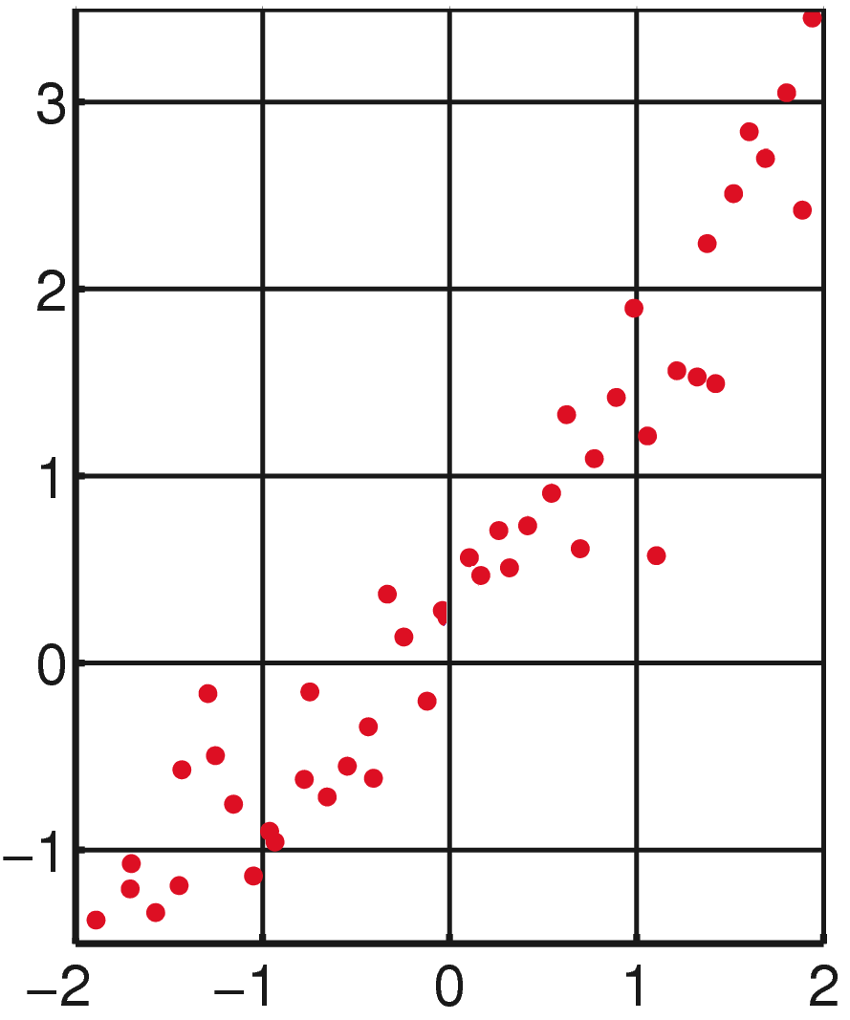
\includegraphics[width=\textwidth]{../images/regression-linear-least-squares-2-only-points.png}}
            \only<2->{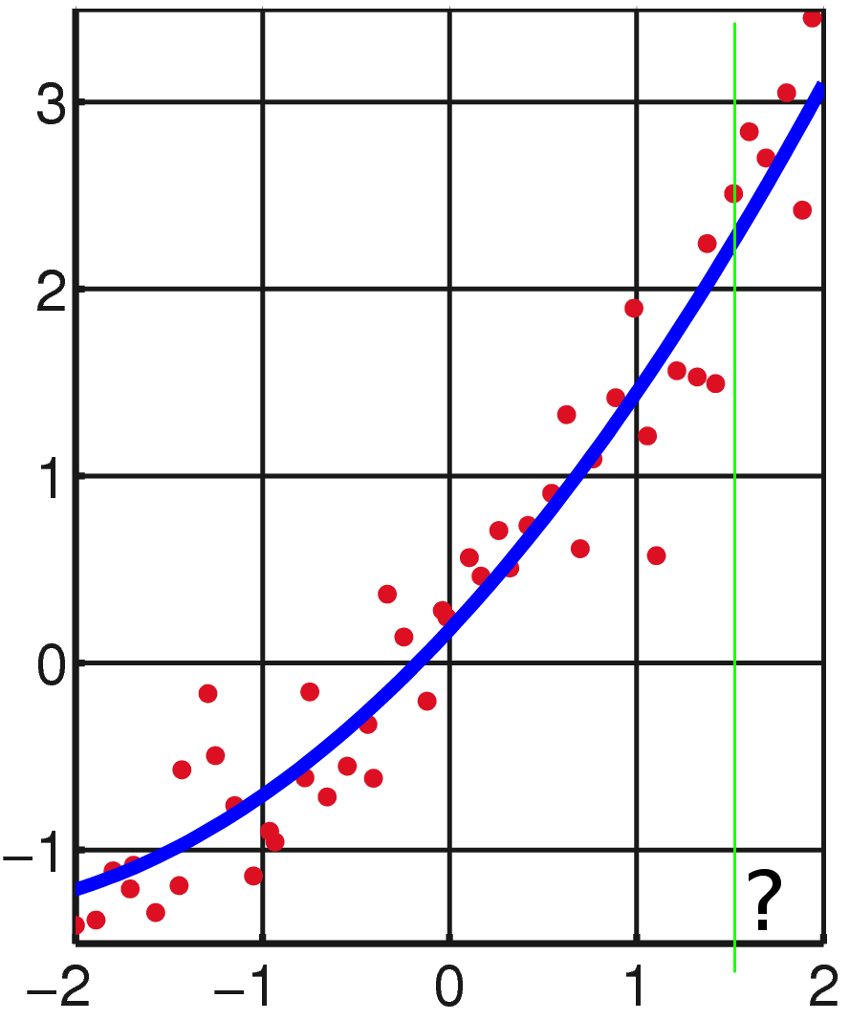
\includegraphics[width=\textwidth]{../images/regression-linear-least-squares-2.png}}
            \caption{Regression}
            \label{fig:Regression}
        \end{minipage}
        \hspace{0.5cm}
        \begin{minipage}[b]{0.45\linewidth}
            \centering
            %\only<1>{
\includegraphics[width=\textwidth]{../images/classification-empty.png}}
            %\only<2>{
\includegraphics[width=\textwidth]{../images/classification-empty.png}}
            \only<3>{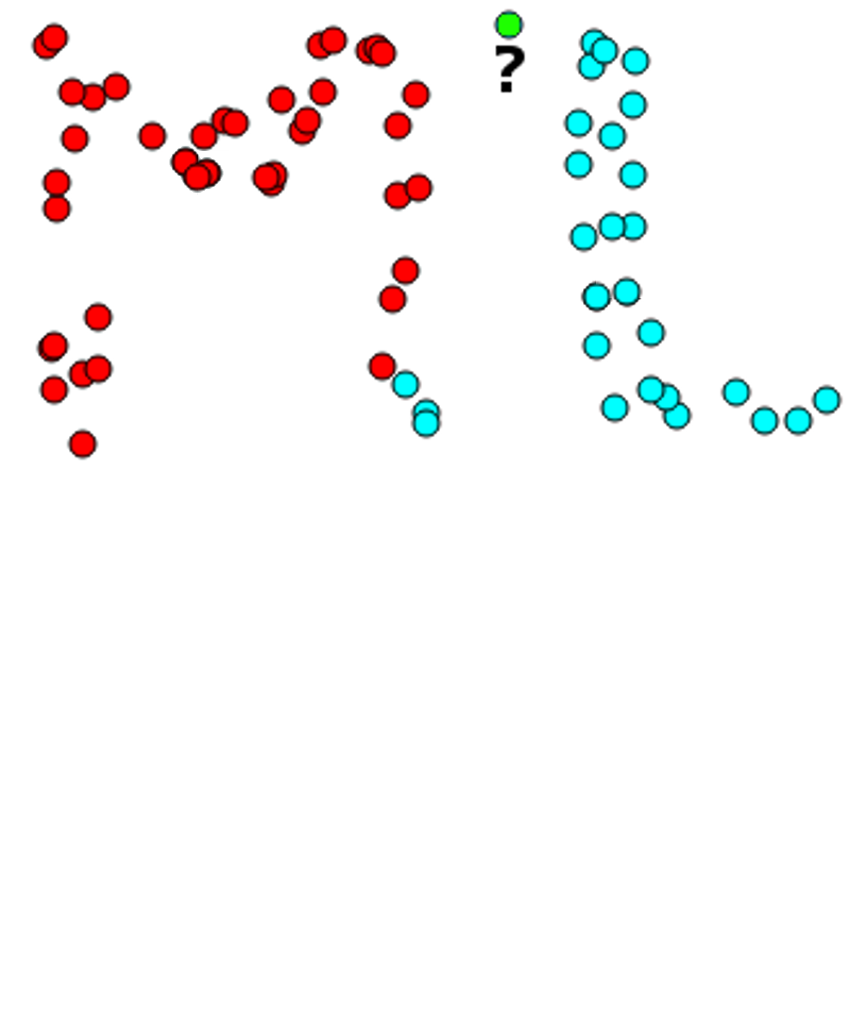
\includegraphics[width=\textwidth]{../images/classification-only.png}}
            \only<4->{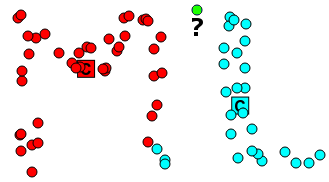
\includegraphics[width=\textwidth]{../images/clustering.png}}
            \caption{\only<-3>{Klassifikation (überwacht)}\only<4->{und Clustering (unüberwacht)}}
            \label{fig:Klassifikation}
        \end{minipage}
    \end{figure}
\end{frame}


\begin{frame}{MNIST - Ziffern klassifizieren}
    \begin{figure}[ht]
        \begin{minipage}[b]{0.45\linewidth}
            \begin{itemize}
                \item Klassen: 0, 1, 2, 3, 4, 5, 6, 7, 8, 9
                \item \num{60000} Trainigsdaten, \num{10000} Testdaten
                      auf \href{http://yann.lecun.com/exdb/mnist/}{yann.lecun.com/exdb/mnist}
                \item Algorithmen zur Klassifizierung: \textbf{SVMs} (Support Vector Machines),
                      \textbf{CNNs} (Convolutional Neural Networks),
                      $k$~Nearest Neighbors (siehe \href{http://martin-thoma.com/k-nearest-neighbor-classification-interactive-example/}{tinyurl.com/knn-interact})
            \end{itemize}
        \end{minipage}
        \hspace{0.5cm}
        \begin{minipage}[b]{0.45\linewidth}
            \begin{figure}
                \centering
                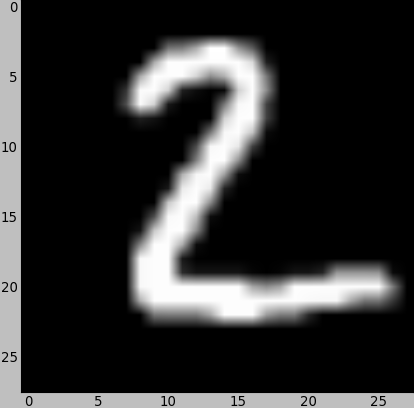
\includegraphics[width=\textwidth]{../images/mnist-2.png}
                \caption{Datensatz der Klasse \enquote{2}; $\SI{28}{\pixel} \times \SI{28}{\pixel}$}
                \label{fig:spline}
            \end{figure}
        \end{minipage}
    \end{figure}
\end{frame}

\begin{frame}{Daten}
    \begin{itemize}
        \item In der Klassifikation:
              Tupel $(X, y)$, wobei $X \in \mathbb{R}^n$ ein Feature-Vektor, $y \in \Set{1, \dots, k}$ das Label und $k$ die Anzahl der Klassen ist.
        \item Skalenniveaus
            \begin{itemize}
                \item Nominal: Namen, Geschlecht
                \item Ordinal: Konfektionsgrößen
                \item Intervall: Anfangszeit einer Veranstaltung
                \item Verhältnis: Temperatur in K
                \item Absolut: Anzahl Personen
            \end{itemize}
        \item Datenmenge: \enquote{There is no data like more data}
    \end{itemize}

    vgl. Vorlesung \enquote{Mustererkennung}
\end{frame}

\begin{frame}{Preprocessing / Feature extraction}
    \begin{itemize}
        \item Wie bekomme ich meine Features?
        \item Bilder: Pixel-Werte für jeden Farbkanal
        \begin{itemize}
            \item Kleiner Skalieren? Rotieren?
            \item Farbraum? (z.B. RGB, HSV, HSL, HSI)
            \item Normalisieren auf $[0, 1]$
        \end{itemize}
        \item Verhältis zweier Größen
        \item Deep Learning: Auto-Encoder
    \end{itemize}

    vgl. Vorlesung \enquote{Neuronale Netze}
\end{frame}

\begin{frame}{Generalisierung und Overfitting}
    \begin{figure}[ht]
        \begin{minipage}[b]{0.45\linewidth}
            \begin{itemize}
                \item Generalisierung: Wie gut ist man auf ungesehenen Daten?
                \item Overfitting: Auswendig lernen
            \end{itemize}

\begin{table}
    \begin{tabular}{cl|ll}
    \toprule
    ~          & ~       & \multicolumn{2}{c}{Trainingsfehler}\\
    ~          & ~       & \Frowny      & \Smiley     \\\midrule
    \multirow{2}{*}{\rotatebox[origin=c]{90}{\parbox{0.9cm}{Test-\newline fehler}}} & \Frowny & Klassifizierer; mehr Trainingsdaten & Overfitting \\
    ~          & \Smiley & Programmierfehler                                     & Perfekt     \\
    \bottomrule
    \end{tabular}
\end{table}
        \end{minipage}
        \begin{minipage}[b]{0.45\linewidth}
        \begin{figure}[H]
            \centering
            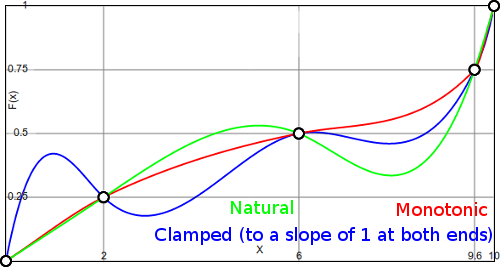
\includegraphics[width=\textwidth]{../images/ancillary-conditions-splines-results.png}
            \caption{5~Datenpunkte, 3~perfekte Modelle}
            \label{fig:mnist-2}
        \end{figure}
        \vspace{2.2cm}
        \end{minipage}
    \end{figure}
\end{frame}

\section{Tools}
\subsection{sklearn}
\framedgraphic{sklearn}{../images/peekaboo-vision-blogspot-de.png}

\subsection{Lasagne}
\begin{frame}{Lasagne}
    \begin{itemize}
        \item Neuronale Netze trainieren
        \item Mit GPU, falls CUDA installiert ist
        \item \href{https://github.com/Lasagne/Lasagne}{github.com/Lasagne}
        \item \href{http://martin-thoma.com/lasagne-for-python-newbies}{Lasagne for Python Newbies}
    \end{itemize}
\end{frame}


\section{Weiteres}
\subsection{Anwendungen}
\begin{frame}{Anwendungen}
    \begin{figure}[ht]
        \begin{minipage}[b]{0.45\linewidth}
            \begin{itemize}
                \item \href{https://how-old.net}{how-old.net}
                \item \enquote{Gelöste} Aufgaben:
                \begin{itemize}
                    \item Gesichter in Bild finden,\\
                          z.B. mit Sliding Window
                    \item Geschlecht klassifizieren: \male, \female
                    \item Regression beim Alter
                \end{itemize}
            \end{itemize}
            \vspace{2cm}
        \end{minipage}
        \hspace{0.5cm}
        \begin{minipage}[b]{0.45\linewidth}
            \centering
            \only<1>{
                \begin{figure}[H]
                    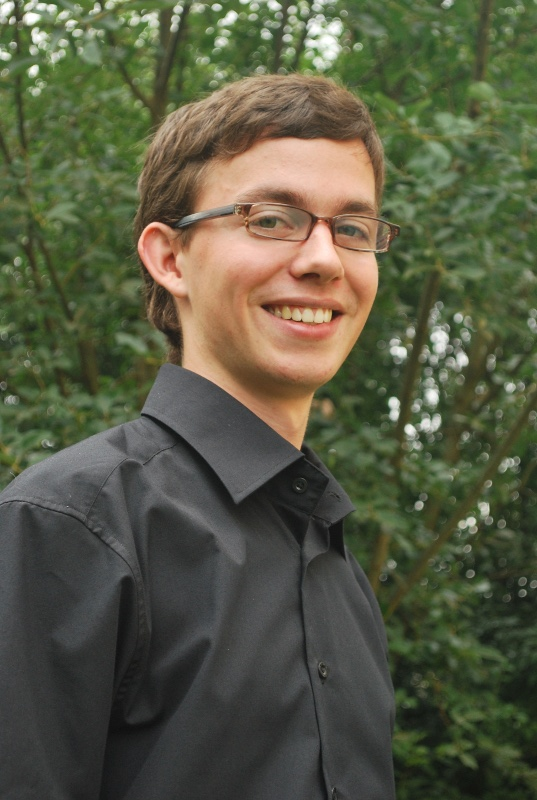
\includegraphics[height=4cm]{../images/Martin-Thoma-web.jpg}
                    \caption{Wie alt bin ich auf diesem Bild?}
                    \label{fig:Klassifikation}
                \end{figure}
            }
            \only<2>{
                \begin{figure}[H]
                    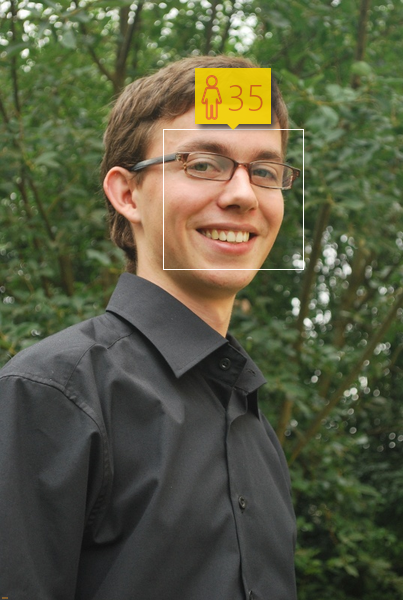
\includegraphics[height=4cm]{../images/Martin-Thoma-how-old.png}
                    \caption{20 Jahre alt}
                    \label{fig:Klassifikation}
                \end{figure}
            }
        \end{minipage}
    \end{figure}
\end{frame}
